
%% bare_conf.tex
%% V1.3
%% 2007/01/11
%% by Michael Shell
%% See:
%% http://www.michaelshell.org/
%% for current contact information.
%%
%% This is a skeleton file demonstrating the use of IEEEtran.cls
%% (requires IEEEtran.cls version 1.7 or later) with an IEEE conference paper.
%%
%% Support sites:
%% http://www.michaelshell.org/tex/ieeetran/
%% http://www.ctan.org/tex-archive/macros/latex/contrib/IEEEtran/
%% and
%% http://www.ieee.org/

%%*************************************************************************
%% Legal Notice:
%% This code is offered as-is without any warranty either expressed or
%% implied; without even the implied warranty of MERCHANTABILITY or
%% FITNESS FOR A PARTICULAR PURPOSE!
%% User assumes all risk.
%% In no event shall IEEE or any contributor to this code be liable for
%% any damages or losses, including, but not limited to, incidental,
%% consequential, or any other damages, resulting from the use or misuse
%% of any information contained here.
%%
%% All comments are the opinions of their respective authors and are not
%% necessarily endorsed by the IEEE.
%%
%% This work is distributed under the LaTeX Project Public License (LPPL)
%% ( http://www.latex-project.org/ ) version 1.3, and may be freely used,
%% distributed and modified. A copy of the LPPL, version 1.3, is included
%% in the base LaTeX documentation of all distributions of LaTeX released
%% 2003/12/01 or later.
%% Retain all contribution notices and credits.
%% ** Modified files should be clearly indicated as such, including  **
%% ** renaming them and changing author support contact information. **
%%
%% File list of work: IEEEtran.cls, IEEEtran_HOWTO.pdf, bare_adv.tex,
%%                    bare_conf.tex, bare_jrnl.tex, bare_jrnl_compsoc.tex
%%*************************************************************************

% *** Authors should verify (and, if needed, correct) their LaTeX system  ***
% *** with the testflow diagnostic prior to trusting their LaTeX platform ***
% *** with production work. IEEE's font choices can trigger bugs that do  ***
% *** not appear when using other class files.                            ***
% The testflow support page is at:
% http://www.michaelshell.org/tex/testflow/



% Note that the a4paper option is mainly intended so that authors in
% countries using A4 can easily print to A4 and see how their papers will
% look in print - the typesetting of the document will not typically be
% affected with changes in paper size (but the bottom and side margins will).
% Use the testflow package mentioned above to verify correct handling of
% both paper sizes by the user's LaTeX system.
%
% Also note that the "draftcls" or "draftclsnofoot", not "draft", option
% should be used if it is desired that the figures are to be displayed in
% draft mode.
%
\documentclass[10pt, conference, compsocconf]{IEEEtran}
% Add the compsocconf option for Computer Society conferences.
%
% If IEEEtran.cls has not been installed into the LaTeX system files,
% manually specify the path to it like:
% \documentclass[conference]{../sty/IEEEtran}





% Some very useful LaTeX packages include:
% (uncomment the ones you want to load)


% *** MISC UTILITY PACKAGES ***
%
%\usepackage{ifpdf}
% Heiko Oberdiek's ifpdf.sty is very useful if you need conditional
% compilation based on whether the output is pdf or dvi.
% usage:
% \ifpdf
%   % pdf code
% \else
%   % dvi code
% \fi
% The latest version of ifpdf.sty can be obtained from:
% http://www.ctan.org/tex-archive/macros/latex/contrib/oberdiek/
% Also, note that IEEEtran.cls V1.7 and later provides a builtin
% \ifCLASSINFOpdf conditional that works the same way.
% When switching from latex to pdflatex and vice-versa, the compiler may
% have to be run twice to clear warning/error messages.






% *** CITATION PACKAGES ***
%
%\usepackage{cite}
% cite.sty was written by Donald Arseneau
% V1.6 and later of IEEEtran pre-defines the format of the cite.sty package
% \cite{} output to follow that of IEEE. Loading the cite package will
% result in citation numbers being automatically sorted and properly
% "compressed/ranged". e.g., [1], [9], [2], [7], [5], [6] without using
% cite.sty will become [1], [2], [5]--[7], [9] using cite.sty. cite.sty's
% \cite will automatically add leading space, if needed. Use cite.sty's
% noadjust option (cite.sty V3.8 and later) if you want to turn this off.
% cite.sty is already installed on most LaTeX systems. Be sure and use
% version 4.0 (2003-05-27) and later if using hyperref.sty. cite.sty does
% not currently provide for hyperlinked citations.
% The latest version can be obtained at:
% http://www.ctan.org/tex-archive/macros/latex/contrib/cite/
% The documentation is contained in the cite.sty file itself.






% *** GRAPHICS RELATED PACKAGES ***
%
\ifCLASSINFOpdf
  % \usepackage[pdftex]{graphicx}
  % declare the path(s) where your graphic files are
  % \graphicspath{{../pdf/}{../jpeg/}}
  % and their extensions so you won't have to specify these with
  % every instance of \includegraphics
  % \DeclareGraphicsExtensions{.pdf,.jpeg,.png}
\else
  % or other class option (dvipsone, dvipdf, if not using dvips). graphicx
  % will default to the driver specified in the system graphics.cfg if no
  % driver is specified.
  % \usepackage[dvips]{graphicx}
  % declare the path(s) where your graphic files are
  % \graphicspath{{../eps/}}
  % and their extensions so you won't have to specify these with
  % every instance of \includegraphics
  % \DeclareGraphicsExtensions{.eps}
\fi
% graphicx was written by David Carlisle and Sebastian Rahtz. It is
% required if you want graphics, photos, etc. graphicx.sty is already
% installed on most LaTeX systems. The latest version and documentation can
% be obtained at:
% http://www.ctan.org/tex-archive/macros/latex/required/graphics/
% Another good source of documentation is "Using Imported Graphics in
% LaTeX2e" by Keith Reckdahl which can be found as epslatex.ps or
% epslatex.pdf at: http://www.ctan.org/tex-archive/info/
%
% latex, and pdflatex in dvi mode, support graphics in encapsulated
% postscript (.eps) format. pdflatex in pdf mode supports graphics
% in .pdf, .jpeg, .png and .mps (metapost) formats. Users should ensure
% that all non-photo figures use a vector format (.eps, .pdf, .mps) and
% not a bitmapped formats (.jpeg, .png). IEEE frowns on bitmapped formats
% which can result in "jaggedy"/blurry rendering of lines and letters as
% well as large increases in file sizes.
%
% You can find documentation about the pdfTeX application at:
% http://www.tug.org/applications/pdftex





% *** MATH PACKAGES ***
%

\usepackage[cmex10]{amsmath}
\usepackage{tikz}

\definecolor{bluekeywords}{rgb}{0,0,1}
\definecolor{greencomments}{rgb}{0,0.5,0}
\definecolor{redstrings}{rgb}{0.64,0.08,0.08}
\definecolor{xmlcomments}{rgb}{0.5,0.5,0.5}
\definecolor{types}{rgb}{0.17,0.57,0.68}

\usepackage{listings}
\lstset{language=[Sharp]C,
captionpos=b,
numbers=left, %Nummerierung
numberstyle=\tiny, % kleine Zeilennummern
frame=lines, % Oberhalb und unterhalb des Listings ist eine Linie
showspaces=false,
showtabs=false,
breaklines=true,
showstringspaces=false,
breakatwhitespace=true,
escapeinside={(*@}{@*)},
commentstyle=\color{greencomments},
morekeywords={partial, var, value, get, set},
keywordstyle=\color{bluekeywords},
stringstyle=\color{redstrings},
basicstyle=\scriptsize,
}

\usepackage[]{algorithm}
\usepackage{algorithmic}
\usepackage{etoolbox}
\usepackage{subfig}


\newcommand{\algorithmicdoinparallel}{\textbf{do in parallel}}
\makeatletter
\AtBeginEnvironment{algorithmic}{%
  \newcommand{\FORALLP}[2][default]{\ALC@it\algorithmicforall\ #2\ %
    \algorithmicdoinparallel\ALC@com{#1}\begin{ALC@for}}%
}
\makeatother


% correct bad hyphenation here
\hyphenation{op-tical net-works semi-conduc-tor}

\newtheorem{theorem}{Theorem}[section]
\newtheorem{lemma}[theorem]{Lemma}
\newtheorem{proposition}[theorem]{Proposition}
\newtheorem{corollary}[theorem]{Corollary}
\newtheorem{property}[theorem]{Property}
\newtheorem{definition}[theorem]{Definition}
\newtheorem{remark}[theorem]{Remark}
\newtheorem{assumption}[theorem]{Assumption}

\newcommand{\norm}[1]{\left\lVert#1\right\rVert}


\begin{document}
%
% paper title
% can use linebreaks \\ within to get better formatting as desired
\title{Acoustic fall detection with Bootstrap Aggregating classifiers}


% author names and affiliations
% use a multiple column layout for up to two different
% affiliations

\author{\IEEEauthorblockN{Loukas Kominis}
\IEEEauthorblockA{
Department of ECE, \\
University of Patras,\\
 Patras, Greece\\
loukaskom@gmail.com}
\and
\IEEEauthorblockN{Yanik Ngoko}
\IEEEauthorblockA{Qarnot computing and University of Paris 13\\
Montrouge, France\\
yanik.ngoko@qarnot-computing.com}
\and
\IEEEauthorblockN{Christophe C\'erin}
\IEEEauthorblockA{University of Paris 13\\
Paris, France\\
christophe.cerin@lipn.univ-paris13.fr}

}

%\author{\IEEEauthorblockN{Yanik Ngoko}
%\IEEEauthorblockA{Qarnot Computing and University of Paris 13\\
%Paris, France\\
%yanik.ngoko@\{qarnot-computing.com, lipn.univ-paris13.fr\}}
%\and
%\IEEEauthorblockN{Christophe C\'erin}
%\IEEEauthorblockA{University of Paris 13\\
%Paris, France\\
%christophe.cerin@lipn.univ-paris13.fr}
%}


% conference papers do not typically use \thanks and this command
% is locked out in conference mode. If really needed, such as for
% the acknowledgment of grants, issue a \IEEEoverridecommandlockouts
% after \documentclass

% for over three affiliations, or if they all won't fit within the width
% of the page, use this alternative format:
%
%\author{\IEEEauthorblockN{Michael Shell\IEEEauthorrefmark{1},
%Homer Simpson\IEEEauthorrefmark{2},
%James Kirk\IEEEauthorrefmark{3},
%Montgomery Scott\IEEEauthorrefmark{3} and
%Eldon Tyrell\IEEEauthorrefmark{4}}
%\IEEEauthorblockA{\IEEEauthorrefmark{1}School of Electrical and Computer Engineering\\
%Georgia Institute of Technology,
%Atlanta, Georgia 30332--0250\\ Email: see http://www.michaelshell.org/contact.html}
%\IEEEauthorblockA{\IEEEauthorrefmark{2}Twentieth Century Fox, Springfield, USA\\
%Email: homer@thesimpsons.com}
%\IEEEauthorblockA{\IEEEauthorrefmark{3}Starfleet Academy, San Francisco, California 96678-2391\\
%Telephone: (800) 555--1212, Fax: (888) 555--1212}
%\IEEEauthorblockA{\IEEEauthorrefmark{4}Tyrell Inc., 123 Replicant Street, Los Angeles, California 90210--4321}}




% use for special paper notices
%\IEEEspecialpapernotice{(Invited Paper)}




% make the title area
\maketitle


\begin{abstract}

We consider the design of an acoustic fall detection system with the Qarnot model of computing. 
Qarnot introduced a computing model based on heaters that embed processors and sensors. 
The network of Qarnot heaters in a home and building offers several advantages for the design of smart-environments 
systems when we consider the privacy, the real-life performance or the acceptance. 
The main goal of this work is to show the effectiveness of this platform for the resolution of smart-home problems  
and acoustic fall detection in particular. 
In addition to consider the Qarnot context, our work also innovates in applying bootstrap aggregation on  
acoustic fall detection. The results we obtained are very encouraging. We were able to build a classifier 
whose accuracy is higher than what we found in the state of the art on the problem. Finally, though the results were obtained in 
using Qarnot tools for the design of smart-environment systems, they can be generalized to other contexts.
\end{abstract}

\begin{IEEEkeywords}
acoustic fall detection; smart-environment; bootstrap aggregation

\end{IEEEkeywords}


% For peer review papers, you can put extra information on the cover
% page as needed:
% \ifCLASSOPTIONpeerreview
% \begin{center} \bfseries EDICS Category: 3-BBND \end{center}
% \fi
%
% For peerreview papers, this IEEEtran command inserts a page break and
% creates the second title. It will be ignored for other modes.
\IEEEpeerreviewmaketitle


\section{Introduction}
\label{introduction}

The demographic explosion of the eldery is offering and unprecendented opportunity for the development of a
assisted living technologies. However, the question of the right architecture for such technologies is critical. 
By the past, several concerns were raised on existing solutions. The sensitive topics include the privacy, 
the acceptance or the real-life performance of such technologies. For the interested reader, we recommend 
the work of Igual et al.~\cite{Igual2013}. 

This work intends to contribute to the design of a fall detection system for elders. Our conviction is 
that with the Qarnot model of computing~\footnote{www.qarnot-computing.com}, it is possible to formulate 
fall detection systems where several of the  classical concerns regarding assisted living technologies are 
addressed. Qarnot introduced a utility computing model where the computing nodes are heaters that are 
embedded in homes, offices, buildings where they serve to heat. These special computing nodes (called Q.rads) 
embed several processors but also sensors related for instance to humidity, $\mathrm{CO2}$, noise, presence 
etc. The heaters are connected to the Internet and at the upper level, the network 
of geo-distributed Q.rads is exploited as an HPC cloud infrastructure (See Figure~\ref{fig:digital}). At the scale of homes 
and buildings in which the Q.rads are deployed, this network serves as a smart-building platform with services like 
the analysis of the air quality or the detection of the sounds of fire-alarms. For more details about the Qarnot model, 
we refer the interested reader to~\cite{DBLP:conf/europar/Ngoko16}.

	\begin{figure}[hbtp]
	\centering
        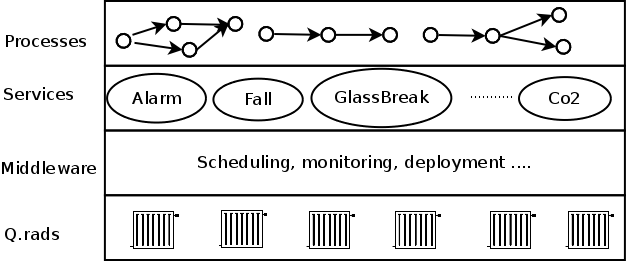
\includegraphics[scale=0.27]{./Figures/layer.png}
	%}
	\caption{Layers of Qarnot smart-homes}
	\label{fig:layer}
	\end{figure}


	\begin{figure*}[htbp]
	\subfloat[{\scriptsize A Q.rad}]{
            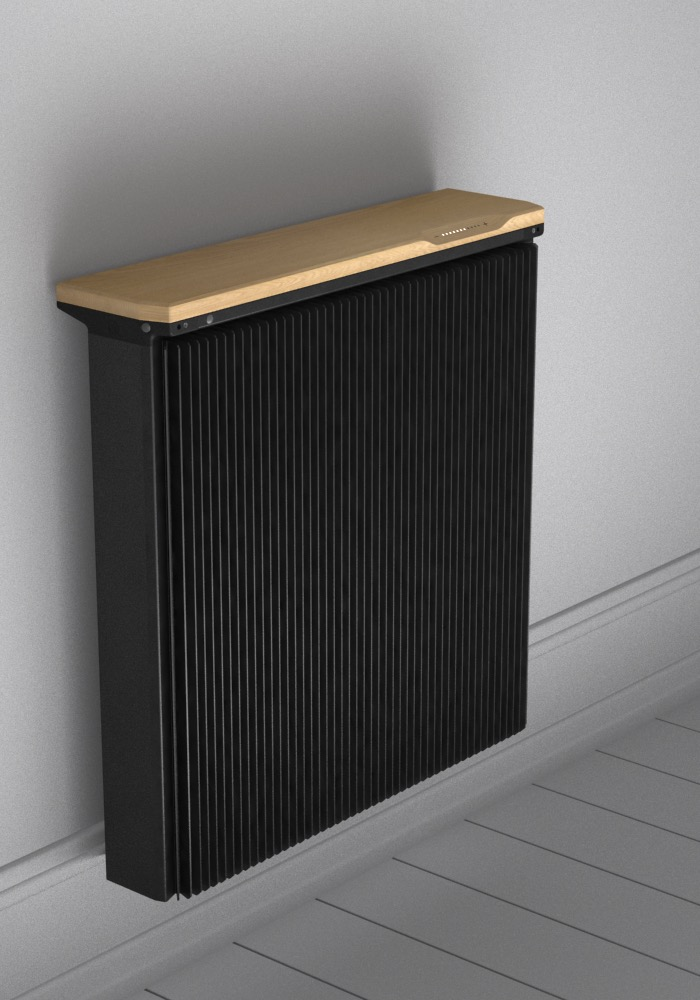
\includegraphics[width=4cm,height=3.7cm]{./Figures/qrad.jpg}
         }
	\subfloat[{\scriptsize The Qarnot model for HPC-cloud}]{
            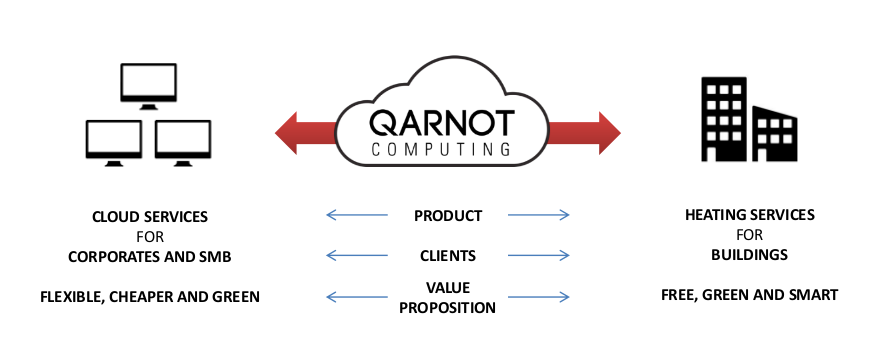
\includegraphics[width=10.7cm,height=3.7cm]{./Figures/model.png}
        }
	\caption{The Qarnot model}
	\label{fig:digital}
	\end{figure*}

In the Qarnot vision, a smart-home is a computing environment whose layered architecture is depicted in Figure~\ref{fig:layer}. 
The architecture includes 4 layers: the processes of the smart-home, the services used to compose the processes, 
the smart-home middleware and the Q.rads.
The smart-home processes implement the intelligent behaviors of the homes. The processes are built in composing the services of 
the environment with the input data flow that are collected either from the Q.rads or from external sensors. An 
example of service is an alarm detection system, a fall detection, glassbreak detection etc. An example 
of process is a flow that collects data from a Q.rad, routes the data to an alarm service 
and then sends an SMTP notification if an alarm is found. The main role of the middleware is to orchestrate 
the smart-home processes on the Q.rads. The middleware also includes a storage system for keeping the data collected 
in a home inside its building. 

Regarding data privacy, this architecture can guarantee that the data collected in a building will not be sent 
in another site. This changes from classical cloud-based smart-homes where the data are saved remotely in a datacenter. 
Regarding acceptance by elders, the Qarnot solution does not require neither a wearable device, nor a smartphone. 
The user does not even need to care about the functioning of their heater. Finally for real-life performance, because of the sensing and 
computing power of the heaters~\footnote{ A heater could embed $4$ processors}, we have enough computing power to locally 
calibrate a machine learning model, for the specific environment in which we operate.
In this paper, we will present the results we got on a distributed training system (machine learning system), 
we designed in order to detect falls with the Qarnot model of computing. 

The automatic fall detection is an old smart-home topic. Several machine learning systems were already 
proposed for its resolution. A good survey on the diverse contributions can be found in~\cite{Igual2013,Mubashir:2013:SFD:2397722.2397898}. 
Despite the interest and quality of these solutions, our work has some specificities that were not addressed in past 
works. Indeed, past systems were often based on videos, accelerometers or smart-phones while we are mainly based on 
acoustic data. The choice to consider acoustic inputs comes from the fact that the Qarnot heaters do not embed cameras. In addition, 
we consider that the solution of an accelerometer or a smart-phone is not efficient in the viewpoint of the acceptance or 
usability by the elders. 

Acoustic fall detection systems were considered in the past. For instance, we can refer to the work of Xiaodan Zhuang~\cite{Xiaodan2009} where GMM and SVM classifier were used and they managed to achieve a fall accuracy of 59\% and 67\% respectively with using only a far-field microphone. Other insteresting works on this field are the ones of Yun et al~\cite{Yun2012} and Muhammad et al~\cite{Muhammad2014} that use audio data to achieve classification of falls, each of them in a specific way.  

Differently to these works, we innovate in two points. The first is that we designed a training system to run on 
the Qarnot system. This was achieved in using the Software Defined Kit of Qarnot to build a solution that is orchestrated by 
the Q.ware resource manager. The second point is that differently from existing works, we used the  bootstrap aggregation. 

Bootstrap aggregating, also known as bagging, is a machine learning ensemble meta-algorithm which was designed to improve the stability and accuracy of machine learning algorithms by combining classifications of randomly generated training sets. Bagging can reduce variance and help to avoid the problem of overfitting. Usually it is applied to decision tree methods, but it can be applied to any method. The usage of this technique leads to an important finding: we were able to build a meta-classifier, 
largely more accurate than all the other classifiers taken separately. We even obtained accuracy and True positive scores that 
we did not find in the literature. 

The remainder of this paper is organized as follows. In Section~\ref{Related}, we present the related works. Section~\ref{Smart} 
present the Qarnot architecture for smart-homes. We detail here the architectural context in which we want to develop a fall 
detection system. Section~\ref{Fall} discusses of the training of a fall detection system with three classifiers: SVM, KNN and decision tree. 
In Section~\ref{BaggingFall} we reconsider the question with Bagging. In Section~\ref{Conclusion}, we conclude.

\section{Related Works} \label{Related}

Given a flow of data related to an environment, the objective of a fall detection system is to state whether or not 
there is a fall we can distinguish from the data flow. To collect the data, we assume that the environment 
is equiped with sensors; depending on their number, dispositions and types, the construction of the fall detection system 
could be more or less challenging. 

For the reader interested in a global summary of fall systems, we recommend the 
work of Igual et al.~\cite{Igual2013}. In particular, this work discusses of the interest in fall detection system for assistive 
living technologies. An interesting point this work mentions is the need of developing fall detection systems of high accuracy 
because of the fear of falling. For elders, the fear of falling  can be more frequent, after a fall incident. According to 
researches~\cite{FearofFalling} this fear has negative consequences to everyday life of people, in many ways. The presence or use of a fall detector though could improve people confidence and feel of security. 

The work of Igual et al. also proposed an effective classification of fall detection systems. Here, two categories are 
distinguished: context-aware systems (without wearables) and systems based on wearable devices. Context-aware systems are built with 
{\it stationary} sensors like cameras, pressure sensors, microphones, infrared sensors. Wearables-based systems are in most cases 
designed with accelerometers. For both of these categories, there are some disadvantages regarding the acceptance of the system. 
For instance, people might not agree on the idea of continuously wearing an extra device inside their home. In the same way, 
privacy concerns might be raised against the usage of a camera. 
Our approach belongs to the category of context-aware systems and the sensors used by our system are the microphones embedded in the Q.rads. 

Fall detection systems based on acoustic data were already proposed in the past. Khan et al~\cite{Muhammad2014}, proposed a 
system to detect fall based on footstep acoustic data (microphones deployed in the floor). In their work, noises interference and 
source separation is an important pre-processing stage. The proposed system is based on Mel-frequency cepstral coefficients (MFCC) 
features, Nearest neighbor and one class support vector machine (OCSVM) for classification. As this work, we will use MFCCs, 
but our data are not collected from sensors located in the floor. Moreover, we will consider other types of classifiers. 

Yun Li et al~\cite{Yun2012} proposed a fall detection system based on a circular microphone array of $0.25$ radius, consisting of eight omnidirectional microphones, uniformly distributed. Such circular distribution is important to localize the sound source. The 
system they proposed is also based on MFCC features and Nearest Neighbor classifiers. In our paper, we will not focus on the distribution 
of sound sources; however, such a study could be envisionned because in Qarnot smart-homes, the Q.rads are distributed in different room. 
Instead, we will consider the simple case where we want to distinguish a fall from the sound recorded on a single Q.rad. We intend 
to generalize to several Q.rads in another study.  

In~\cite{Zigel5223652}, the authors proposed a fall detection system based on floor sensors and acceloremeters. The proposed solution  
include two sub-systems: an event detection system followed by event classification. The former sub-system aims at determining 
segments of the acoustic flows that might comprise a fall. These segments are then sent to a Bayes classifier. One specificity 
of the systems is to account on the human voices. For this, the system is trained with a shock sentence pronunced with a fall.
The final system we intend to build share several aspects of the propositions made in~\cite{Zigel5223652}: the need of an audio segmentation 
system, the introduction of shock sentences, the processing based on MFCC features. However, we intend to build such a system with 
the Qarnot architecture. 


The work that we found closer to our is certainly the one of Zhuang et al.~\cite{Zhuang4959522}. The authors showed that in 
combining mixture of gaussians (GMM) and super vector machines (SVM), it is possible to reach an accuracy close to $0.41$ on 
acoustic fall detection. As this work, we assume in our paper that the input audio is given as a segment of $5$ seconds. We also
use a similar model for features and consider that the input audio we process is obtained in combining falls, other significative 
sounds and background noises. However, we differ from this work in the classification technique we use. In particular, we showed 
that better scores could be expected with bootstrap aggregation. 

      
 

\section{Qarnot architecture for smart homes} \label{Smart}

	\begin{figure}[hbtp]
	\centering
        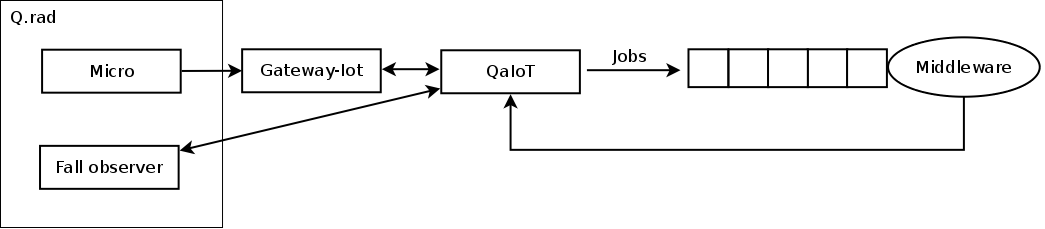
\includegraphics[scale=0.17]{./Figures/gateway.png}
	%}
	\caption{Main components in the processing of acoustic flows for fall detection.}
	\label{fig:flow}
	\end{figure}

In Figure~\ref{fig:flow}, we present the main components in the processing of an acoustic flow recorded in a Qarnot smart-home. 
In this architecture, the fall detection system is composed of two programs: an observer (fall observer) and a fall classifier. 
The observer is a daemon program deployed in Q.rads. It continuously monitors the input acoustic flow to detect falls. 
When it suspects that parts of the flow could include a fall, it segments it in order to have an audio record whose boundaries 
are the begining and the end of the fall. It then initiates the execution of the fall 
classifier on the  audio record. Depending on the result of the fall classifier, the observer will send or not a 
fall notification.  

In this architecture, to access to the microphone data, the observer must first send an HTTP request to QaIot. 
This will cause the registration of the fall observer as an actor to which QaIot must send the data related to microphones. QaIot will 
establish a websocket communication to send these data. The fact that an actor requested data of a microphone will 
oblige the Gateway-Iot to frequently collect acoustic data from microphone. Thus, the fall observer will almost have 
the acoustic data in real-time. 

To detect audio segments with falls, the observer uses a segmentation algorithm. The algorithm frequently computes the energy 
and the frequency of the signal it receives. When these quantities exceed a given value, the 
algorithm will run a pattern detection process to cut a segment that includes probable boundaries of the fall. 
It will then send a request to QaIoT to ask for a deep analysis of the suspected segment. QaIoT will then create a task that 
consists of running the fall classifier on the segment. The created task are next submitted to the Qarnot smart-home middleware. 
If the run of the classifier concludes positively on the occurence of a fall a notification will be sent. In all cases, the 
fall observer will continue to inspect the input flow.

In this model, the run of the fall observer is less compute-intensive than the one of the fall 
classifier. In addition, whereas the fall observer should permanently be executed, the fall classifier could only be launched  
when there is a suspicious audio record. For these reasons, we decide to schedule fall classifier tasks at the middleware 
level where there is a global view of the resource utilization. Our paper will not focus on the fall observer; instead, 
we will consider the design of the fall classifier. In the next section, the framework used for its design will be 
presented. 


\subsection{Framework for classification} 
\begin{figure*}[htbp]
  \captionsetup{aboveskip=-5pt}
	\centering
	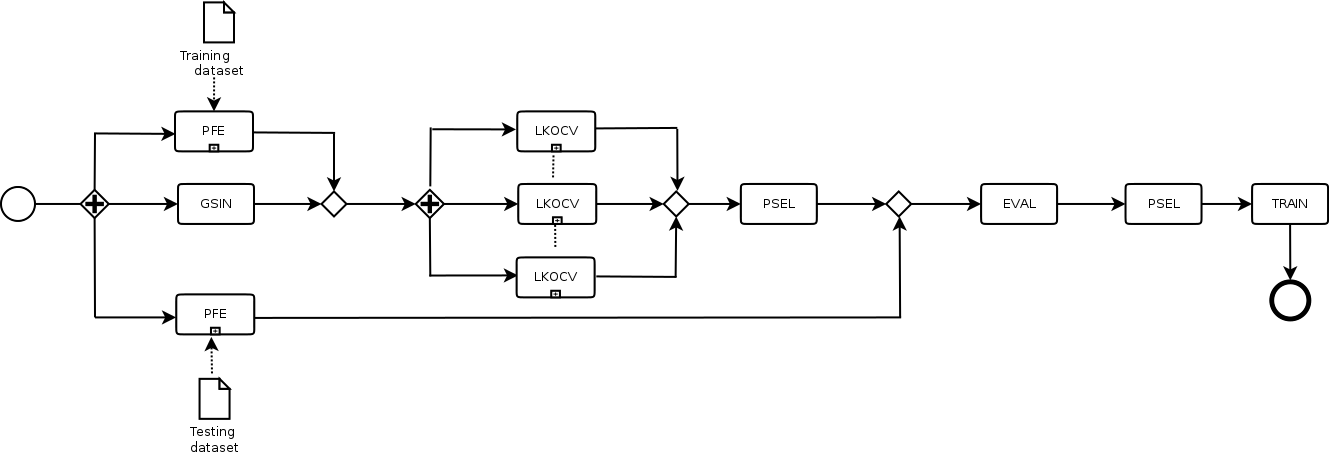
\includegraphics[scale=0.3]{./Figures/workflow.png}
	\caption{Training system}
	\label{fig:training}
	\end{figure*}


Figure~\ref{fig:training} shows the framework we use to build fall classifiers. The representation follows the 
BPMN notations (An empty lozenge is a join and a lozenge with a plus is a fork...). It is important to notice that 
the framework was globally conceived to train 0/1 classifiers from acoustic data issued from Qarnot smart-homes. 
The framework is based on 5 activities and subprocesses that we discuss below.

\begin{itemize}

\item {\bf PFE:} Given a set of wav files, the goal is to extract the acoustic features of the wav files. PFE is a subprocess 
consisting of a set of parallel activities where the acoustic features are separately computed from each dataset file. 
The features we used are the classical ones used in signal processing (Mel-frequency spectrum,energy etc.). Their complete list 
is defined in~\cite{pyAudioAnalysis}.

\item {\bf GSIN:} The framework implements a grid search process whose goal is to find the best classifiers depending on the 
parameters we use. GSIN consists in the initialization of this grid search. It generates configurations of parameters and hyperparameters 
to build the classifier.

\item {\bf LKOCV:} For each input configuration of the grid search, we generate a classifier in learning with 
Leave-k-out cross-validation. The classifiers we considered will be discussed in the next.

\item {\bf PSEL:} From a list of classifiers whose False and True Positive rates (FPR, TPR) are defined (generated in LKOCV or EVAL), we select the ones that are in the Pareto front where we minimize the FPR and maximize the TPR.

\item {\bf EVAL:}  Assuming a list of classifiers and the input features of the testing dataset, we evaluate here the classifiers on the testing features. The TPR and FPR of each classifier are returned.

\item {\bf TRAIN:} We train the selected classifiers with all data from training and testing sets.
\end{itemize}

We implemented this framework as a workflow (based on scikit-learn~\footnote{http://scikit-learn.org}) that can locally (in a home) create jobs associated with these different activities in 
a Qarnot smart-home. The workflow also includes a data collection system that can automatically collect background noises 
from a Qarnot smart-home and then mixes them with fall noises and other significative sounds in order to have a classifier 
that is calibrated for the home in which we are. 
In order to validate the system, we performed various experiments to see if we can create accurate classifiers in 
such a context. The experiments were organized in two series that will be discussed in the next sections.


\section{First serie: building fall classifiers with SVM, KNN and decision trees} \label{Fall}

\subsection{Dataset}

\subsubsection{Falls and significative sounds} 

As already discussed, for training, we considered a basis of audio records that combines: fall noises, significative sounds and 
background noises. To get fall noises and significative sounds, we used an existing dataset~\cite{Dataset} for fall detection. 
This dataset includes $191$ videos with different time durations, from $6$ seconds to $1.20$ minutes. The videos where recorded 
at $25$ frames/s and the resolution is $320 \times 240$ pixels.  Using the Audacity software, we extracted the audios from these videos 
and isolated the fall and no-fall segments. We considered two durations for the extracted segment: $5$ and $10$ seconds. For each of 
these durations, we created a specific dataset. Finally, we applied a re-sampling algorithm in order to have the audio files at 
the same sampling rate ($44100$ Hz).

\subsubsection{Mixture with background noises and features extraction}

Given the fall and no-fall segments, the next stage of the procedure was to mix them with background noises recorded from 
Qarnot-heaters. The input of the mixture procedure was: the audio records of the previous stage, a proportion 
value $p_{fall} \in \{ 0.2, 0.4, 0.5, 0.6 \}$ and a record lenght $T \in \{ 5, 10 \}$. For each assignment of value to $p_{fall}$ and $T$, the mixture procedure generated a dataset of $6400$ records. Here, $p_{fall}$ is the proportion of records that will contain a fall 
and $T$ is the duration of records. For instance, in the case where $p_{fall} = 0.2$ and $T = 10$, we will have a dataset 
of $6400$ records of $10$ seconds with $20$\% of the records corresponding to falls. If the proportion is $0.6$, then we will 
have  $6400$ records that include $60$\% of falls.  On each of these dataset, we then applied a feature extraction algorithm 
to get the MFCCs from the audios. For the extraction, we used the pyAudioAnalysis library~\cite{giannakopoulos2015pyaudioanalysis}. 

\subsubsection{Subsets creation}

The last step in dataset creation is to specify which data will be part of the test dataset and which ones will be used for 
training. On each dataset of $6400$ records, we applied a random partitioning algorithm that assigned $80$\% of the data 
in the train dataset and $20$\% in the test dataset. 

We ran the workflow that implements the framework of Figure~\ref{fig:training} with these different dataset and classifiers. 
As already stated, we used the Scikit-learn implementation of the classifiers. We also used, for cross-validation, the leave-one-out 
method implemented in Scikit-learn. 


\subsection{Experiments plan}


\subsection{SVM and KNN implementation}

After our dataset was fully complete and ready to use in training, SVM and kNN classifiers were implemented on it. In part we present the work done in four experimentation Phases, where the algorithms run in different proportions of data and cover all possible scenarios. The proportion of falls and no falls will be increased and decreased respectively in each Phase in order to check how the algorithms respond on the amount of data given.

The Scikit-Learn python library is used for importing the code, needed for the classifiers, to our main python code. Scikit-Learn library was selected as it provides an easy, universal way for importing different classifiers. 

In each classifier used, after training is finished, which is done using the Q.ware platform and actual Q.rads as computing nodes, the five most efficient classifiers are selected and a choice of the best one is made, among them, based on shortest training time. Because apart from the scores and high accuracy we try to accomplish, a time-efficient method is also important to be created. The most important part is the evaluation of the classifier, where the best classifier is used on both Testing and Training Dataset and see through the Learning Curves and the scores of the confusion matrix, which are presented, how the classifier responds as the amount of data is increasing. 

\subsubsection{Phases workflow and results}

In total our experimental section consists of four Phases. In each of them, a different proportion of fall and no fall data was used in order to check the response of the algorithms. In Table 1, the proportions and total amount of data are presented for each Phase. 

In Phase 1, only SVM classifier is trained and we chose to begin with this specific one as it is mostly used to other researches. The results though were definitely not what we expected as at first True-positive rate is really low and False-positive rate seemed unrealistic as a value. The duration of audio data in this phase (audio segment of fall or no fall mixed with noise) was 10 seconds and proportion of falls and no falls was 20-80\%. 

In Phase 2, it was decided to reduce duration of the audio data to 5 seconds in order to make it easier for the classifier to detect the fall part. It would also improve training time. Falls and no falls proportion was 40-60\%. Also the KNN classifier was introduced and trained for the first try as an effort to compare results with SVM. Better results were produced to the SVM, as the True-positive rate increased by 20\%. KNN had similar scores to the SVM as shown in the table, but in general these results are not yet acceptable in order for our system to be independent. 

So moving on to Phase 3, SVM and KNN classifiers were trained again, duration of audio data is still 5 seconds and proportion of data is changed to 50-50\% and we hoped to improve more the scores of the classifiers. But instead of our expectations for continuous improvement, the SVM results were dissapointing. Not only scores did not icrease but they deteriorated. KNN on the other hand, had better results. This difference in the results can be explained by the different definition of the two classifiers. As KNN detects similarities in a close nearby area it is profited by adding more fall data. In this phase, it was when we first thought of having a different approach on the way of classification, as the system seems to have a kind of sensitivity to the amount of data given each time, that it is not easy to regulate. 

As it was needed to see if our thoughts had logical basis, we moved on to Phase 4. Here, the same settings are used, except the proportion of data used, which changed to 60-40\% of falls and no falls. And the results, certified our theory of sensitivity. The SVM classifier, had a significant improvement and for sure these were the best scores achieved with this specific classifier. KNN still produced good results but not with such a huge improvement to its scores. 

By checking the results shown in Table 2, which presents the scores of each classifier for all four experimentation Phases, the above described are more clear. Three are the categories presented. False-positive-rate (F.P.R), True-positive-rate (T.P.R) and Accuracy.  

\begin{table}[ht]
\caption{\it Proportions of data, for each Phase}
\label{Proportions}
\begin{center}
\begin{small}
\begin{sc}
\begin{tabular}{|l|c|c|c|r|}
\hline
Phase & Fall & Fall(\%) & No Fall & No Fall(\%) \\
      & Samples &        & Samples &            \\ 
\hline
1    & 1600 & 20 & 4800 & 80 \\
\hline
2    & 2400 & 40 & 4000 & 60 \\
\hline
3    & 3200 & 50 & 3200 & 50 \\
\hline
4    & 4000 & 60 & 2400 & 40 \\
\hline
\end{tabular}
\end{sc}
\end{small}
\end{center}
\vskip 0.1in
\end{table}

\begin{table}[t]
\caption{\it Classifiers scores, in each Phase}
\label{Scores}
\vskip 0.1in
\begin{center}
\begin{small}
\begin{sc}
\begin{tabular}{|l|c|c|c|r|}
\hline
Phase & Classifier & F.P.R & T.P.R & Accuracy\\
\hline
Ph.1    & SVM & 0.00 & 0.18 & 0.79 \\
\hline
Ph.2    & SVM & 0.12 & 0.45 & 0.75 \\
     & KNN & 0.10 & 0.42 & 0.73 \\
\hline
Ph.3    & SVM & 0.40 & 0.20 & 0.40 \\
	 & KNN & 0.17 & 0.78 & 0.80 \\
\hline
Ph.4    & SVM & 0.20 & 0.92 & 0.90 \\
	 & KNN & 0.21 & 0.79 & 0.77 \\
\hline
\end{tabular}
\end{sc}
\end{small}
\end{center}
\vskip -0.3in
\end{table}

\subsection{Figures}

Here we present the learning curves for each of the four experimental Phases previously described in order to visualize our results. 
{\bf arrange in correct order figures}


\subsection{Conclusion}

After testing SVM and KNN classifiers in different amount of data and comparing their scores, it is clear that this kind of system behaves differently depending on the amount of data given each time. The SVM results leave no doubt to this statement. KNN has better scores, but as explained previously it is due to the way it works and classifies falls. Our main accomplishment is the one presented on next section.

\section{Second serie: fall detection with bagging} \label{BaggingFall}
 

The results of the previous experimentations, made us considering a different approach for this type of system. The data sensitivity issue had to be solved. So in this Section, a new classifier is introduced in order to help us achieve better scores and easier classification of falls and solve the data sensitivity issue. Bootstrap Aggregating, commonly known as Bagging, is an ensemble meta-estimator. It is important to give an explanation of Bagging in order to make clear for the reader, how we think it can help us. Bagging classifier establishes base estimators to randomly selected subsets of our main dataset. Then it aggregates their estimation to produce one final estimation for the entire dataset. This is its main advantage against other methods. 

The randomly selected subsets assure that we can have an estimation for all possible combinations of data instead of choosing a fixed proportion. Furthermore, the idea of base estimators, aggregated to a final estimation, gives the opportunity to combine all estimations, in an effort to consider parts of the dataset were classification is done properly and other where it is not. 

So this section is also split in Phases. But with some differencies from the previous one. Here proportion of data is kept stable for every Phase and is 50-50\% of falls and no falls, so that we can have enough samples of both categories. The duration of audio data is still 5 seconds. What is getting different at each Phase are the estimators, in an effort to see if we can achieve better results than the classifiers used in previous section. 

\subsection{Decision Tree base estimators}

The first approach of classification with Bagging method was done using it's default parameters which include Decision Tree base estimators. The results produced by our first try were more than satisfying. Actually they were much better than our initial expectations when we considered trying Bootstrap aggregating. Except from the fact that False-positive rate is under 20\%, combined this time with a True-positive rate which significantly increased to 90\%, also Accuracy reached 90\%. The Learning curves of this classifier represent a system with stable improvement as more data were given to it, which is a success for our systems, as it means that by collecting and providing more data to this classifier we can further improve our scores. 

\subsection{KNN base estimators} 

So as the results of the previous Phase were really promising and much better than any previous try, it was decided to make some simulations with other base estimators in order to examine if Bagging can have a positive effect to other classifiers. In this phase, KNN base estimators were selected in an try to see if better results than the KNN classifier alone, can be produced. And the results presented in Table 3, prove that this is a goal that can be achieved with the new method we introduced.   

\subsection{SVM base estimators}

After experimenting on Bagging method with Decision Tree and KNN estimators it was also really important to try it with SVM estimators. We needed to prove that in a fall detection systems were data sensitivity exists, this method can in general improve the scores of single classifiers. So we present the results of Bagging with SVM estimators in Table 3 and as the reader can notice ... {\bf finish after adding SVM results} 

\begin{table}[hb]
\caption{\it Bagging Classifier scores with different estimators}
\vskip 0.1in
\begin{center}
\begin{small}
\begin{sc}
\begin{tabular}{|l|c|c|c|r|}
\hline
Estimator & F.P.R & T.P.R & Accuracy\\
\hline
Decision Tree & 0.16 & 0.90 & 0.87 \\
\hline
KNN & 0.22 & 0.88 & 0.84 \\
\hline
SVM & 0.xx & 0.xx & 0.xx \\
\hline
\end{tabular}
\end{sc}
\end{small}
\end{center}
\vskip -0.2in
\end{table}

\subsection{Figures}

After presenting the scores for each classifier trained, what is also an important tool for machine learning are Learning curves. This section is dedicated to the Learning curves of the classifiers trained during the different phases of this project. 
It is important to see who the system can benefit from adding more data. 
{\bf add the figures of bagging}

\begin{figure}[h]
\vskip 0.2in
\begin{center}
\centerline{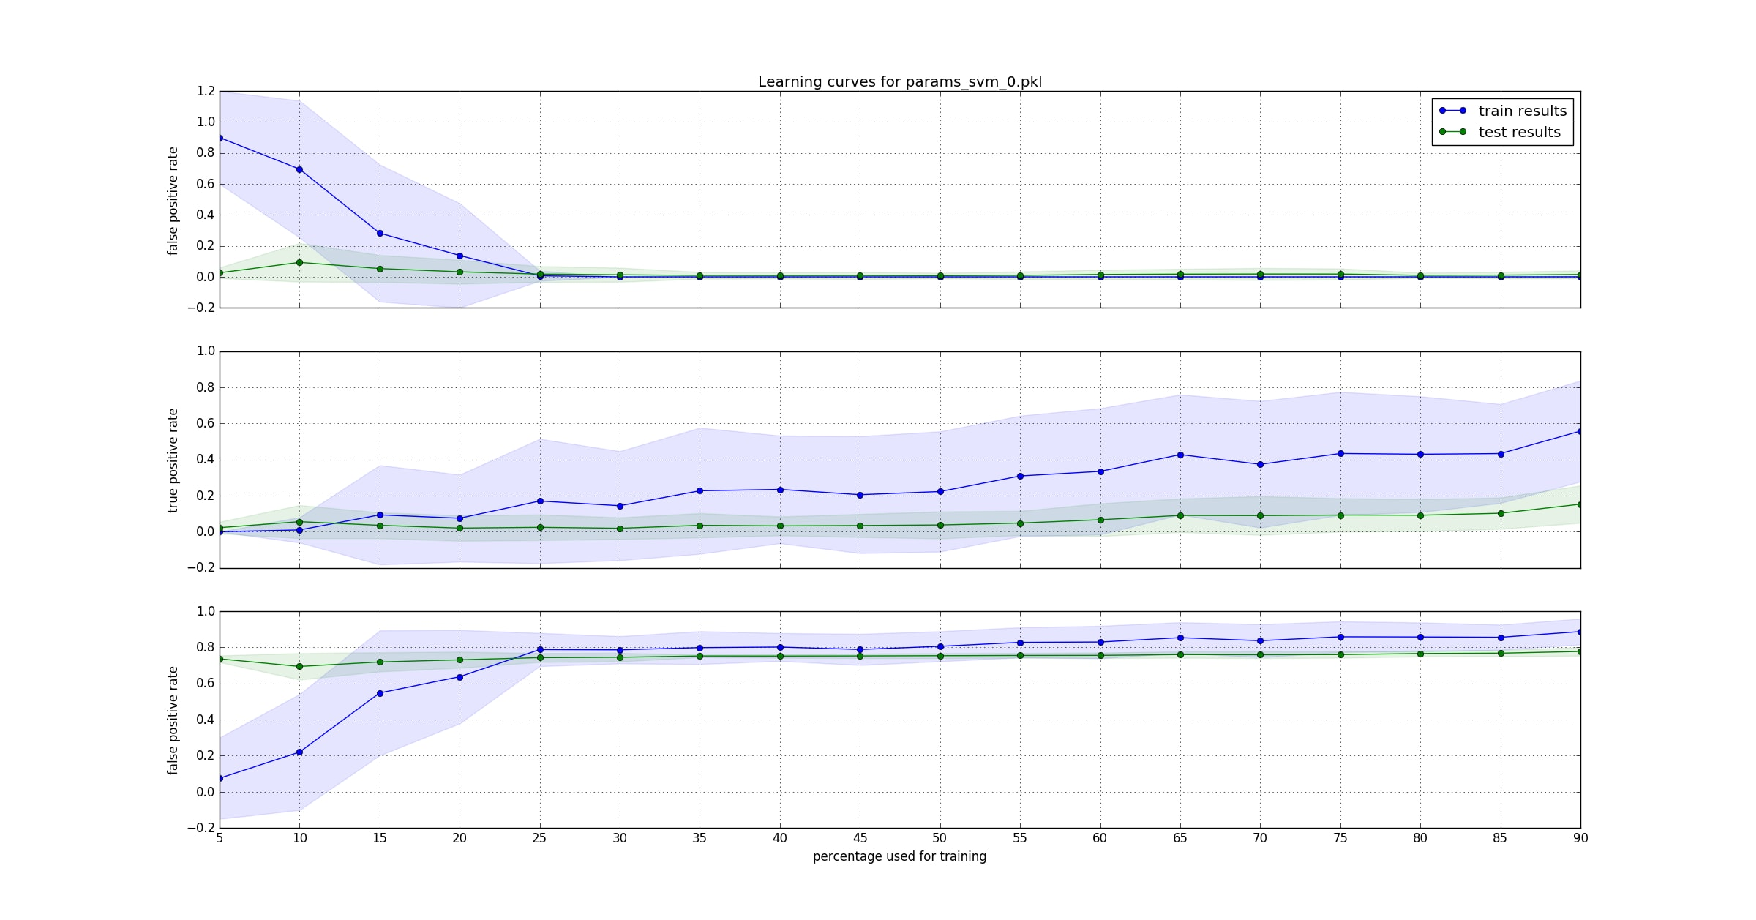
\includegraphics[width=\columnwidth, scale=1]{./Figures/Lc_Ds1_P20-80_SVM}}
\caption{Learning curves, Phase 1, SVM}
\label{learning curves}
\end{center}
\vskip -0.2in
\end{figure} 

\begin{figure}[h]
\vskip 0.2in
\begin{center}
\centerline{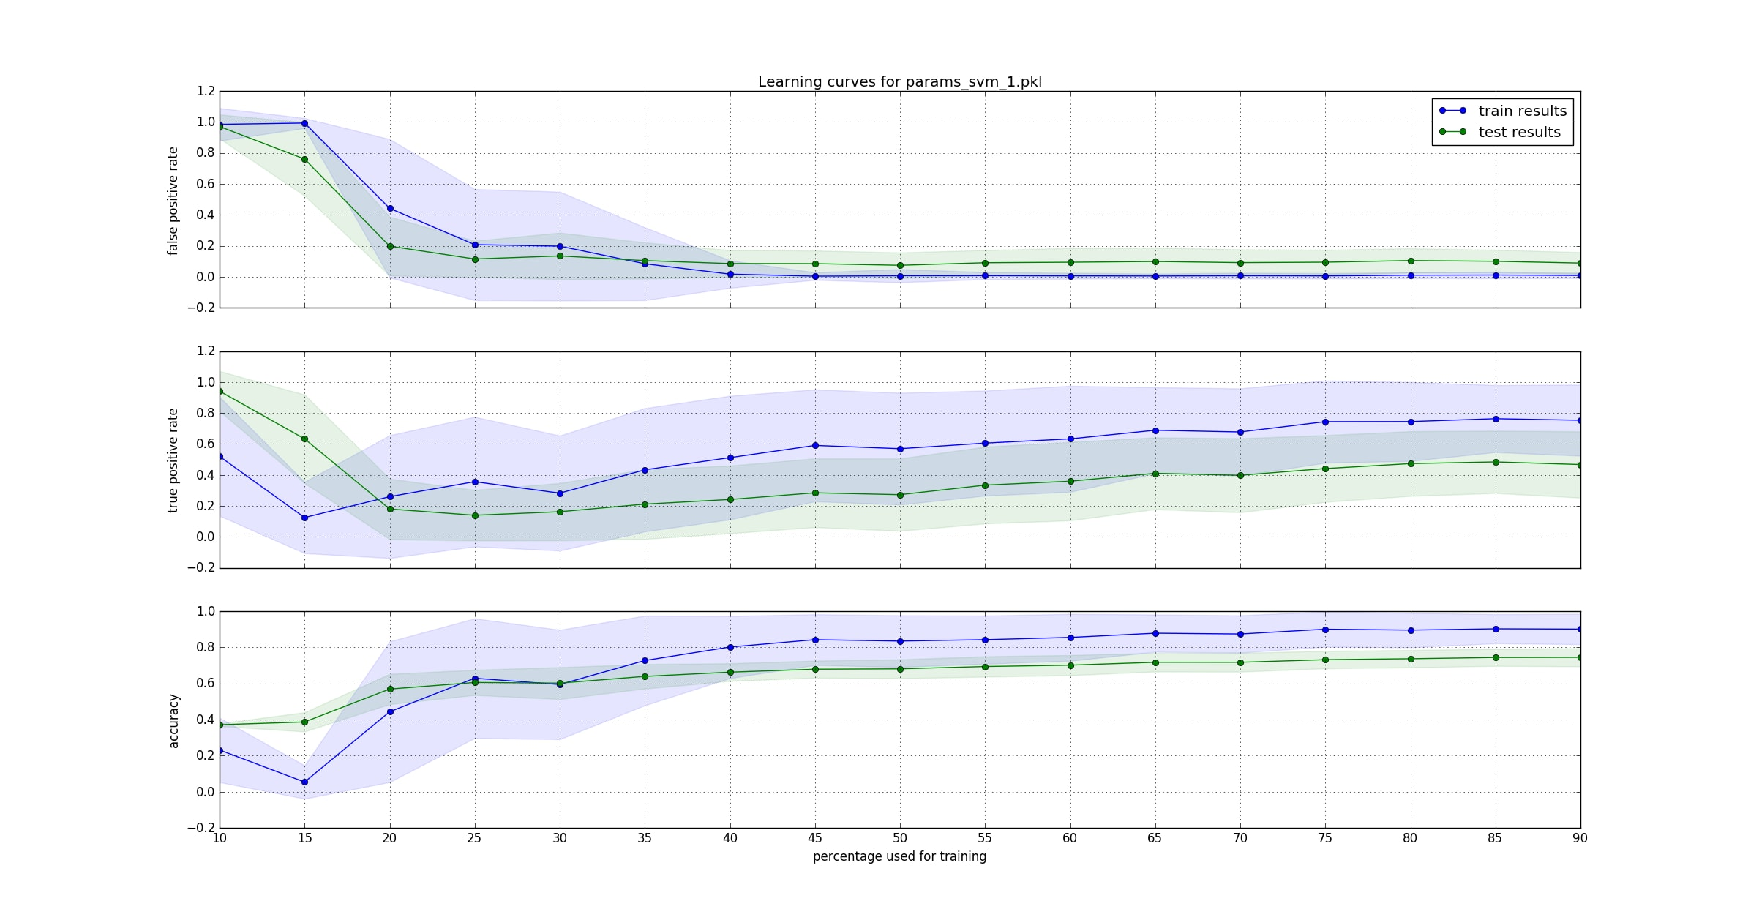
\includegraphics[width=\columnwidth, scale=1]{./Figures/Lc_Ds2_P40-60_SVM}}
\centerline{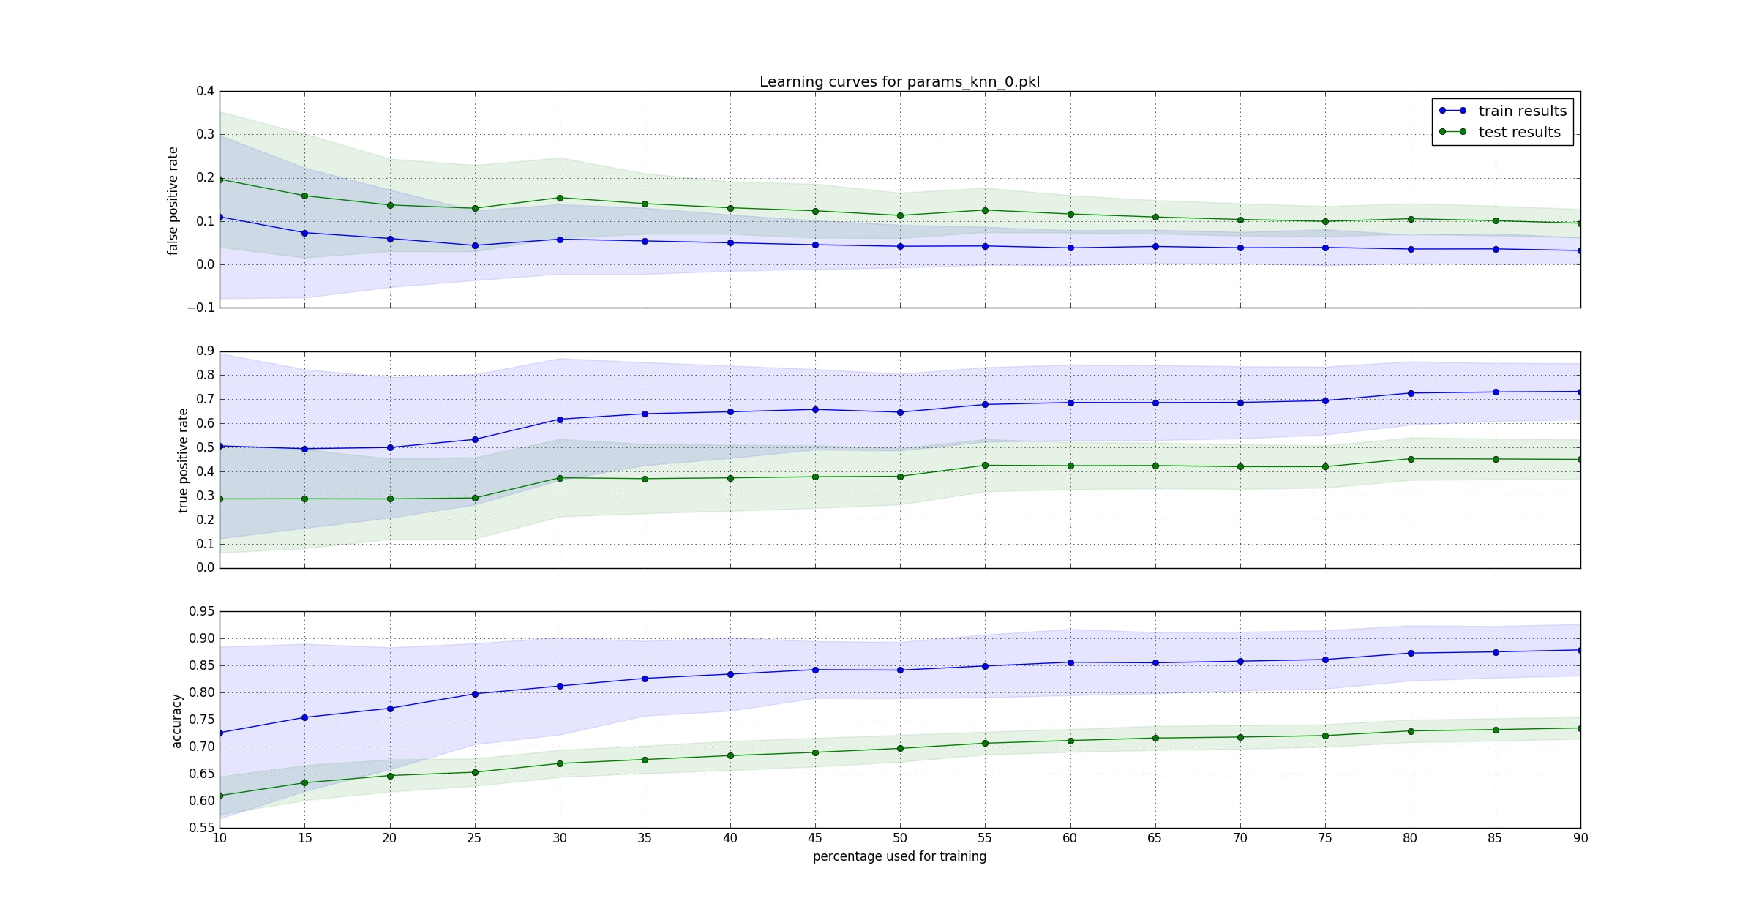
\includegraphics[width=\columnwidth, scale=1]{./Figures/Lc_Ds2_P40-60_kNN}}
\caption{Learning curves, Phase 2, SVM \& and KNN}
\label{learning curves}
\end{center}
\vskip -0.2in
\end{figure} 

\begin{figure}[h]
\vskip 0.2in
\begin{center}
\centerline{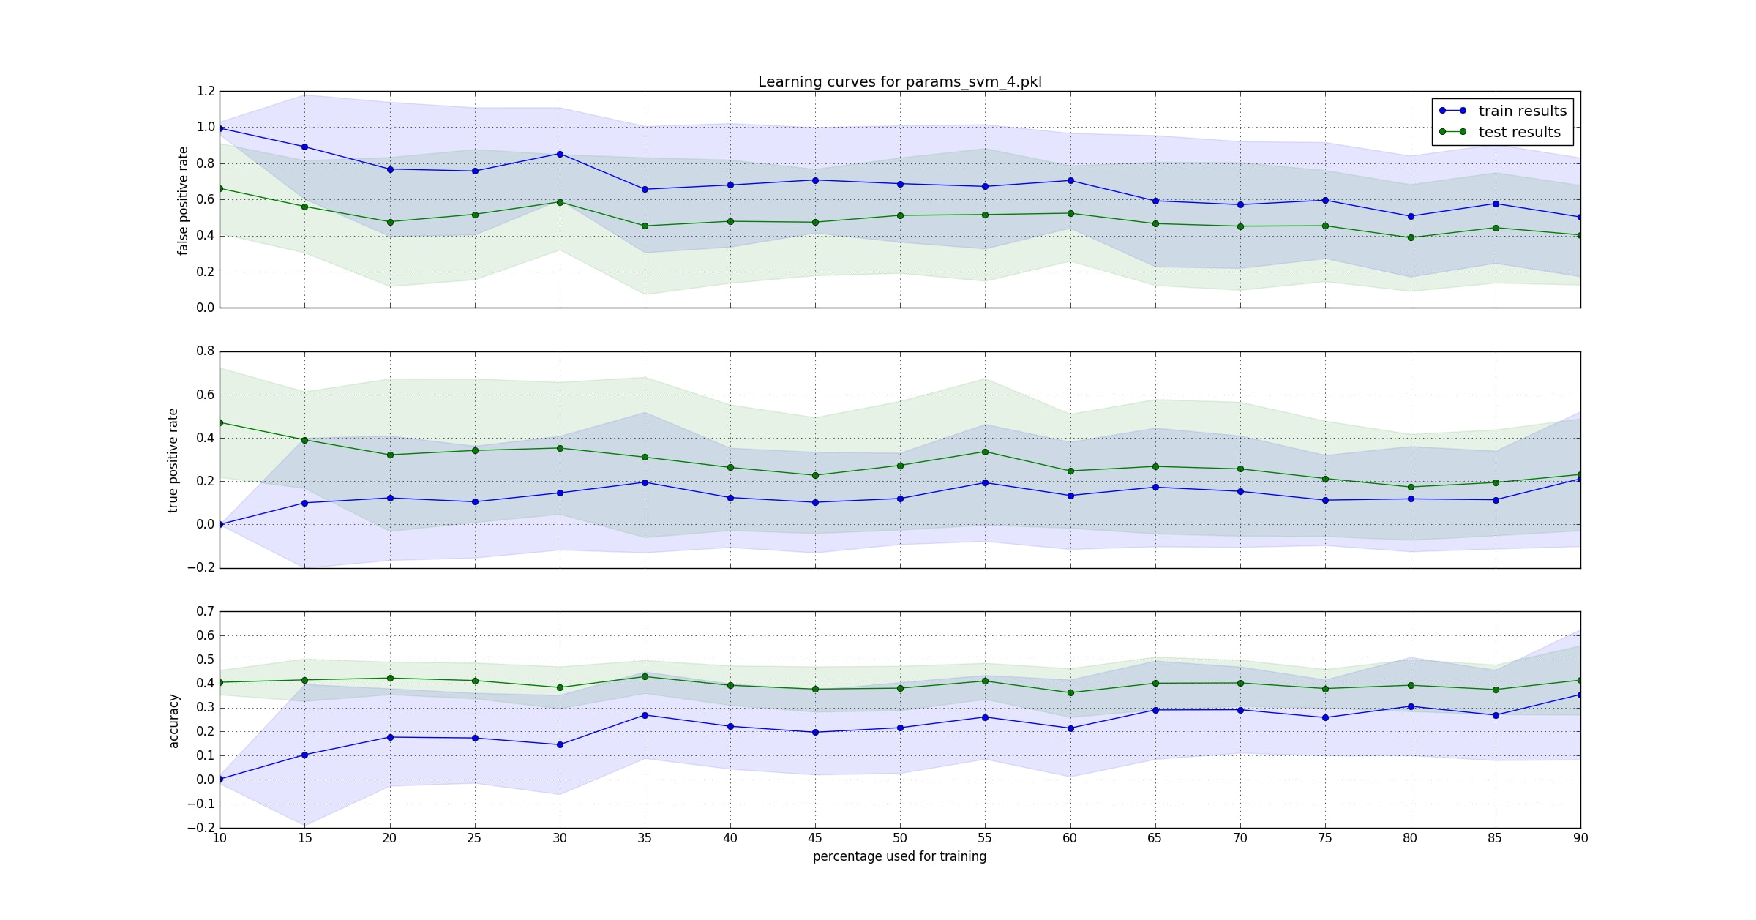
\includegraphics[width=\columnwidth, scale=1]{./Figures/Lc_Ds3_P50-50_SVM}}
\centerline{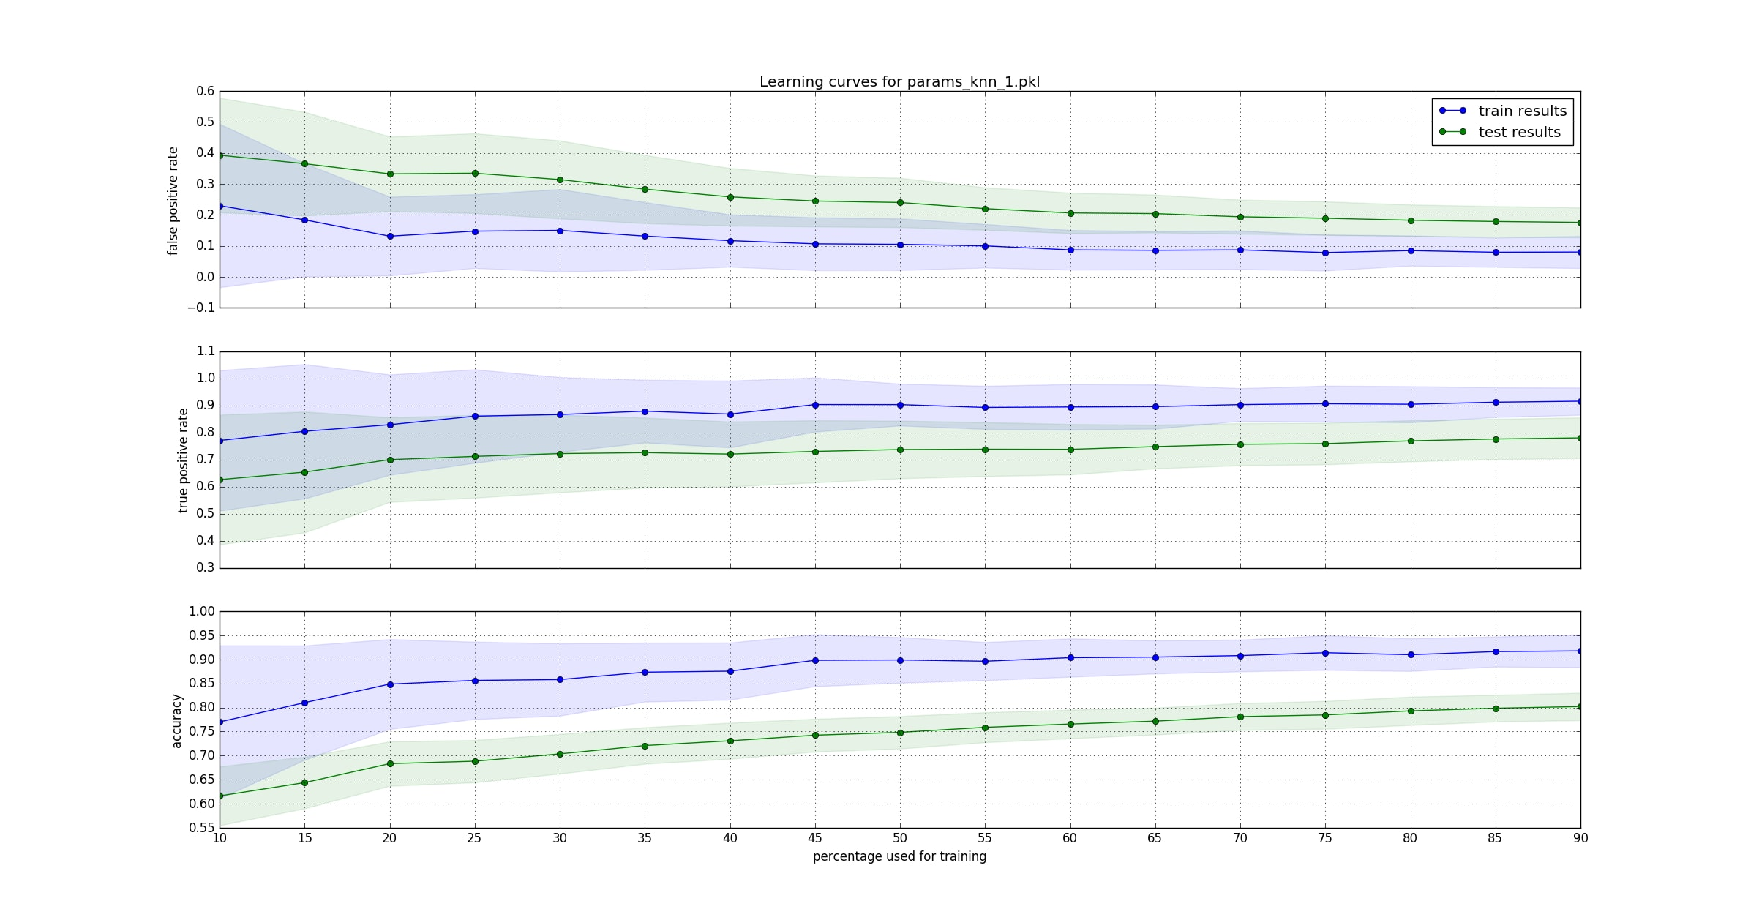
\includegraphics[width=\columnwidth, scale=1]{./Figures/Lc_Ds3_P50-50_kNN}}
\caption{Learning curves, Phase 3, SVM and KNN}
\label{learning curves}
\end{center}
\vskip -0.2in
\end{figure} 

\begin{figure}[h]
\vskip 0.2in
\begin{center}
\centerline{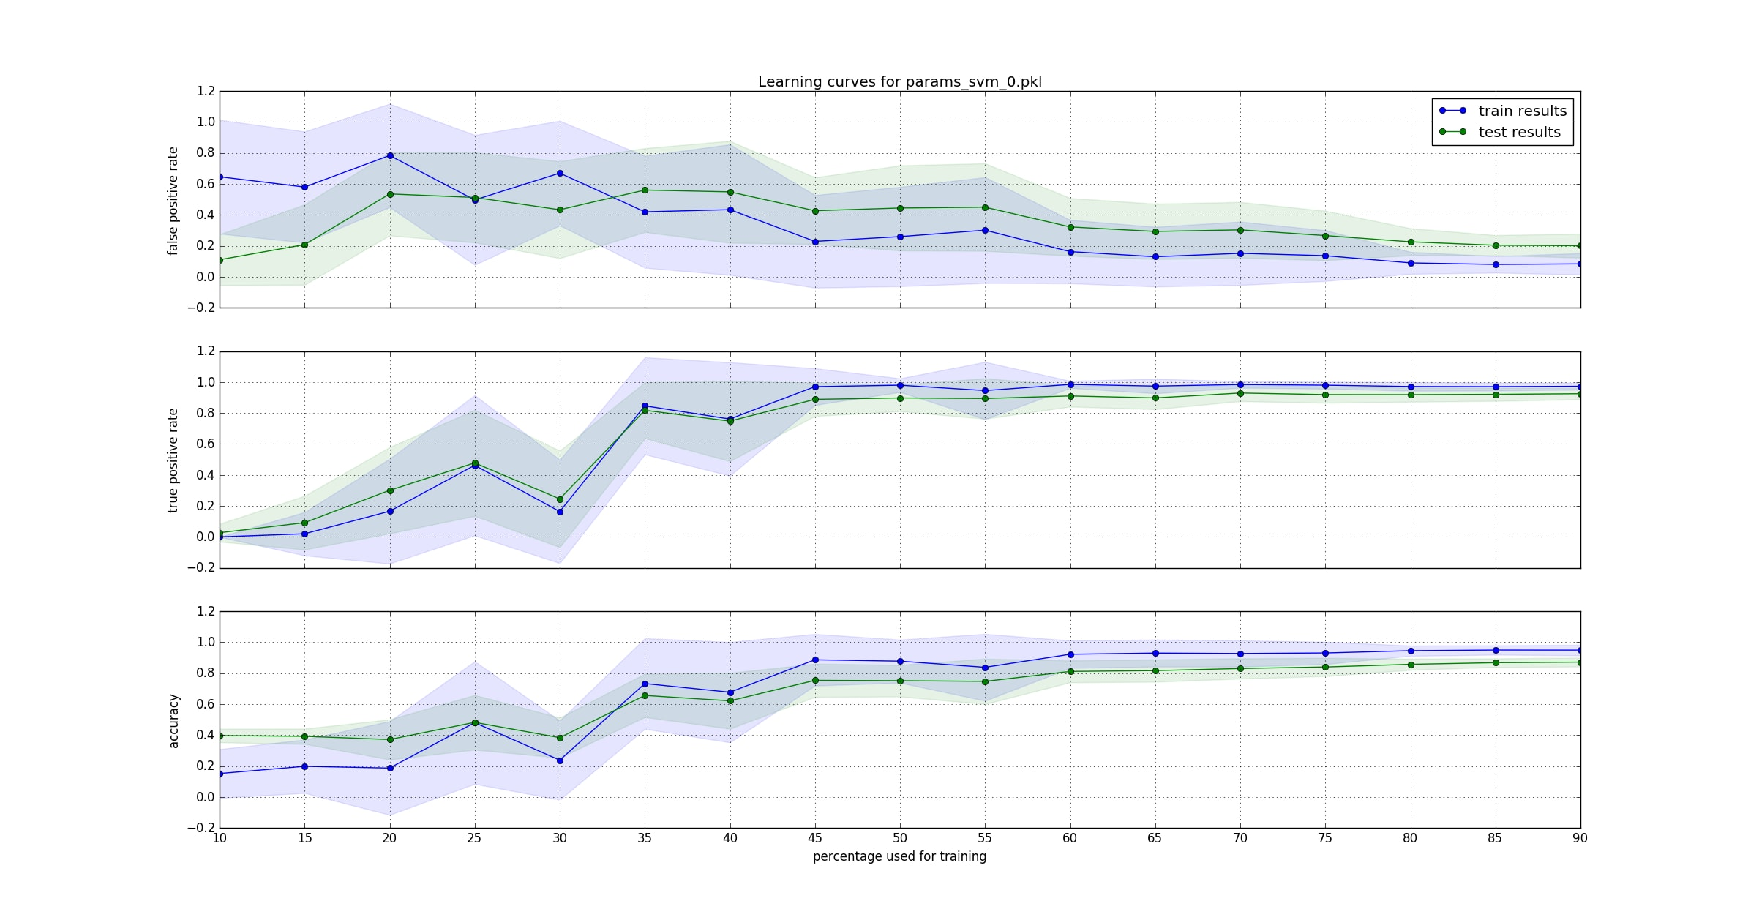
\includegraphics[width=\columnwidth, scale=1]{./Figures/Lc_Ds4_P60-40_SVM}}
\centerline{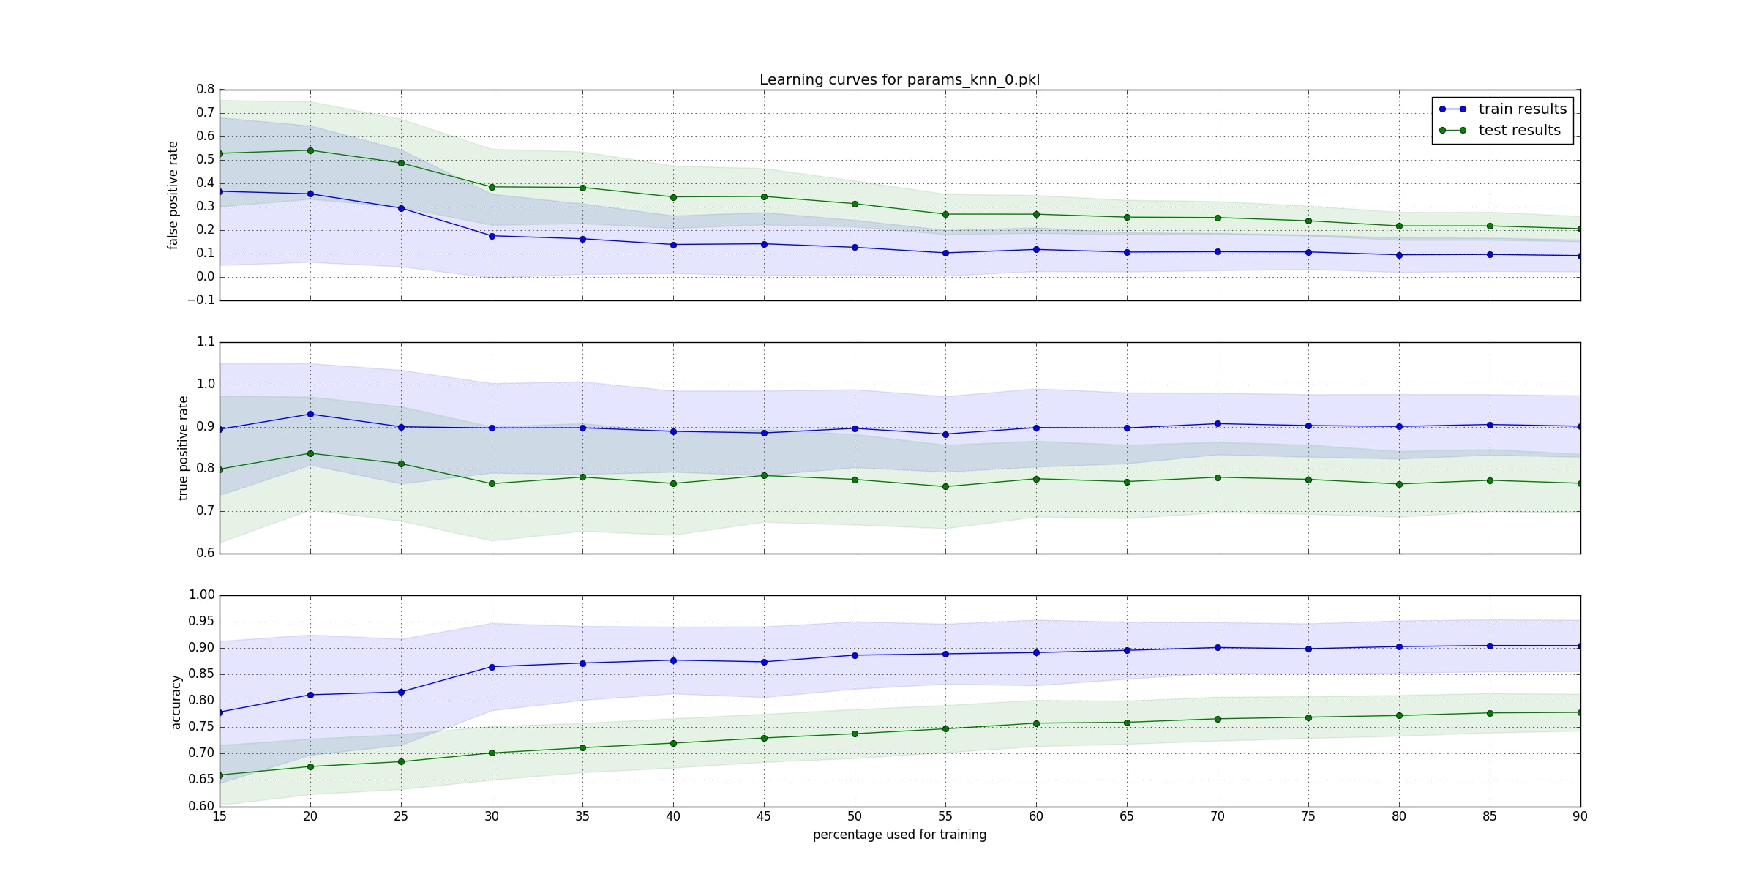
\includegraphics[width=\columnwidth, scale=1]{./Figures/Lc_Ds4_P60-40_kNN}}
\caption{Learning curves, Phase 4, SVM and KNN}
\label{learning curves}
\end{center}
\vskip -0.2in
\end{figure} 


\begin{figure}[h]
\vskip 0.2in
\begin{center}
\centerline{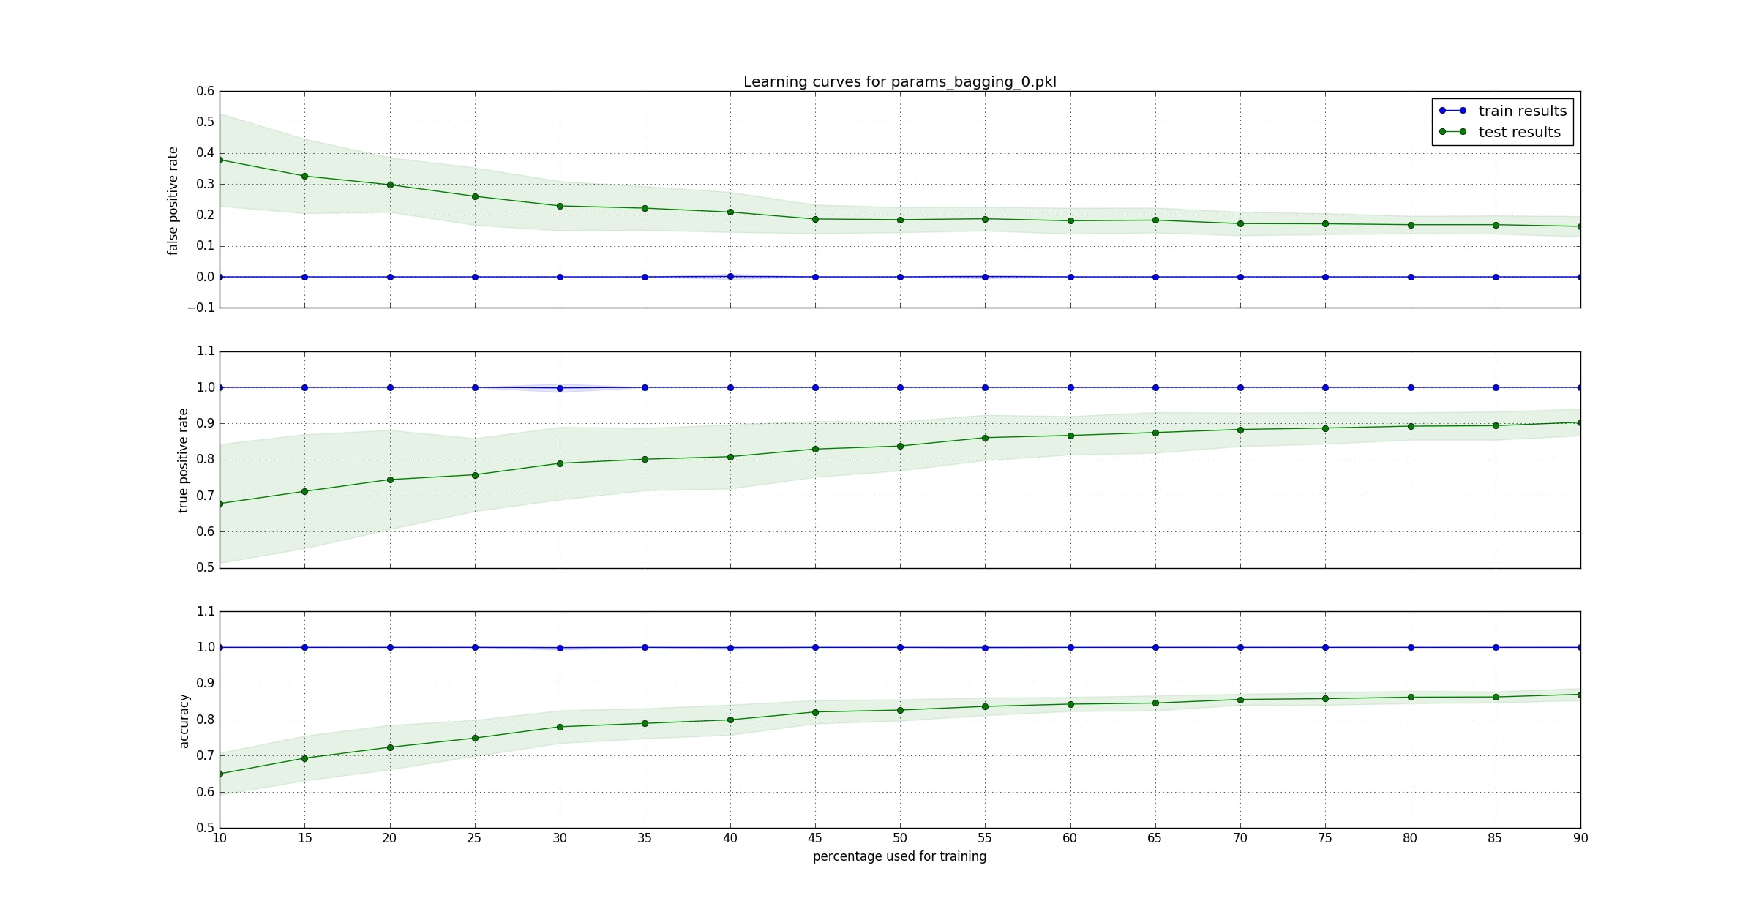
\includegraphics[width=\columnwidth, scale=1]{./Figures/Lc_Ds5_P50-50_BaD}}
\centerline{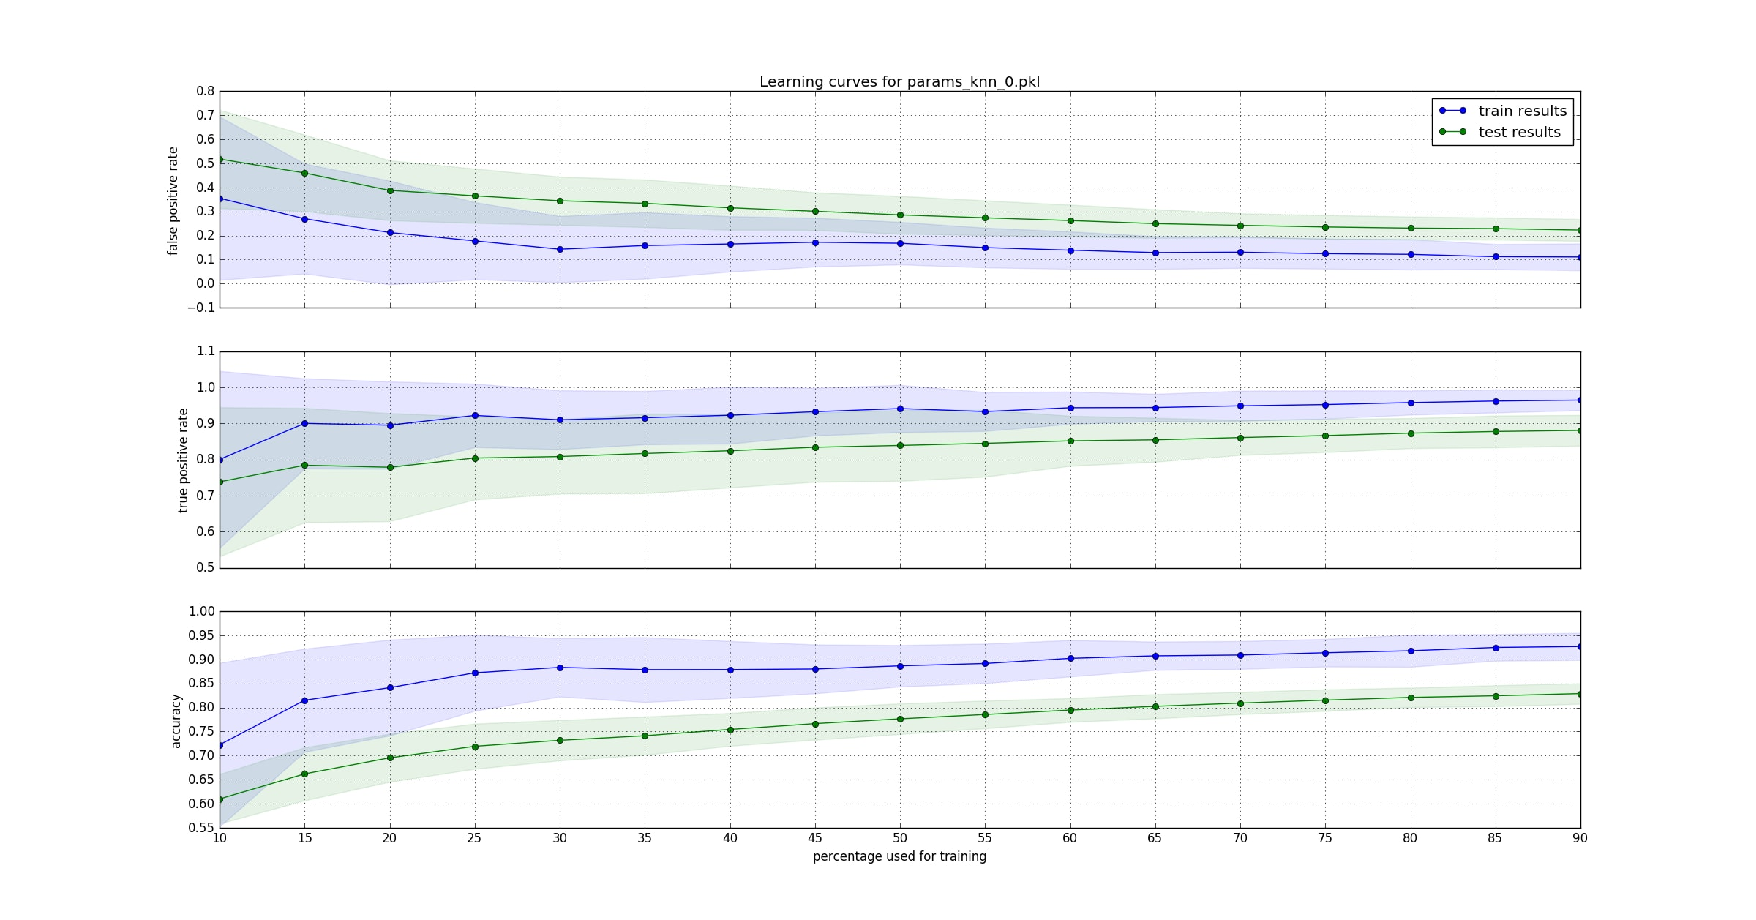
\includegraphics[width=\columnwidth, scale=1]{./Figures/Lc_Ds5_P50-50_Bak}}
\caption{Learning curves, Bagging classifier, Decision Tree, KNN and SVM estimators}
\label{learning curves}
\end{center}
\vskip -0.2in
\end{figure}


\section{Conclusion} \label{Conclusion}

\bibliographystyle{./IEEEtran}
\bibliography{acousticFall}




% that's all folks
\end{document}

